\begin{figure}[htbp]\centering
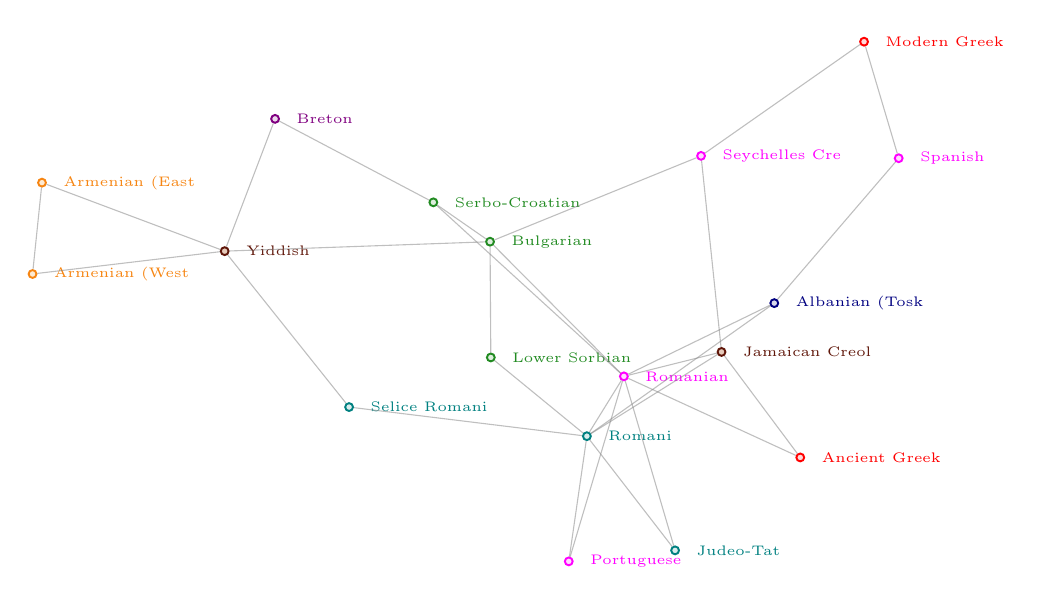
\begin{tikzpicture}[font=\scriptsize]
\node[circle,draw=ForestGreen,fill=ForestGreen!15,line width=0.7pt,inner sep=1pt] (L0) at (0.31,0.76) {};
\node[font=\tiny,ForestGreen,anchor=west] at (0.46,0.76) {Bulgarian};
\node[circle,draw=Magenta,fill=Magenta!15,line width=0.7pt,inner sep=1pt] (L1) at (2.01,-0.95) {};
\node[font=\tiny,Magenta,anchor=west] at (2.16,-0.95) {Romanian};
\node[circle,draw=Red,fill=Red!15,line width=0.7pt,inner sep=1pt] (L2) at (4.25,-1.98) {};
\node[font=\tiny,Red,anchor=west] at (4.40,-1.98) {Ancient Greek};
\node[circle,draw=Teal,fill=Teal!15,line width=0.7pt,inner sep=1pt] (L3) at (2.66,-3.16) {};
\node[font=\tiny,Teal,anchor=west] at (2.81,-3.16) {Judeo-Tat};
\node[circle,draw=ForestGreen,fill=ForestGreen!15,line width=0.7pt,inner sep=1pt] (L4) at (-0.41,1.26) {};
\node[font=\tiny,ForestGreen,anchor=west] at (-0.26,1.26) {Serbo-Croatian};
\node[circle,draw=Magenta,fill=Magenta!15,line width=0.7pt,inner sep=1pt] (L5) at (2.99,1.85) {};
\node[font=\tiny,Magenta,anchor=west] at (3.14,1.85) {Seychelles Cre};
\node[circle,draw=NavyBlue,fill=NavyBlue!15,line width=0.7pt,inner sep=1pt] (L6) at (3.92,-0.02) {};
\node[font=\tiny,NavyBlue,anchor=west] at (4.07,-0.02) {Albanian (Tosk};
\node[circle,draw=BurntOrange,fill=BurntOrange!15,line width=0.7pt,inner sep=1pt] (L7) at (-5.38,1.51) {};
\node[font=\tiny,BurntOrange,anchor=west] at (-5.23,1.51) {Armenian (East};
\node[circle,draw=BurntOrange,fill=BurntOrange!15,line width=0.7pt,inner sep=1pt] (L8) at (-5.50,0.35) {};
\node[font=\tiny,BurntOrange,anchor=west] at (-5.35,0.35) {Armenian (West};
\node[circle,draw=Sepia,fill=Sepia!15,line width=0.7pt,inner sep=1pt] (L9) at (-3.06,0.64) {};
\node[font=\tiny,Sepia,anchor=west] at (-2.91,0.64) {Yiddish};
\node[circle,draw=Purple,fill=Purple!15,line width=0.7pt,inner sep=1pt] (L10) at (-2.42,2.32) {};
\node[font=\tiny,Purple,anchor=west] at (-2.27,2.32) {Breton};
\node[circle,draw=Magenta,fill=Magenta!15,line width=0.7pt,inner sep=1pt] (L11) at (5.50,1.82) {};
\node[font=\tiny,Magenta,anchor=west] at (5.65,1.82) {Spanish};
\node[circle,draw=ForestGreen,fill=ForestGreen!15,line width=0.7pt,inner sep=1pt] (L12) at (0.32,-0.71) {};
\node[font=\tiny,ForestGreen,anchor=west] at (0.47,-0.71) {Lower Sorbian};
\node[circle,draw=Teal,fill=Teal!15,line width=0.7pt,inner sep=1pt] (L13) at (1.54,-1.71) {};
\node[font=\tiny,Teal,anchor=west] at (1.69,-1.71) {Romani};
\node[circle,draw=Red,fill=Red!15,line width=0.7pt,inner sep=1pt] (L14) at (5.06,3.30) {};
\node[font=\tiny,Red,anchor=west] at (5.21,3.30) {Modern Greek};
\node[circle,draw=Magenta,fill=Magenta!15,line width=0.7pt,inner sep=1pt] (L15) at (1.31,-3.30) {};
\node[font=\tiny,Magenta,anchor=west] at (1.46,-3.30) {Portuguese};
\node[circle,draw=Sepia,fill=Sepia!15,line width=0.7pt,inner sep=1pt] (L16) at (3.25,-0.64) {};
\node[font=\tiny,Sepia,anchor=west] at (3.40,-0.64) {Jamaican Creol};
\node[circle,draw=Teal,fill=Teal!15,line width=0.7pt,inner sep=1pt] (L17) at (-1.48,-1.34) {};
\node[font=\tiny,Teal,anchor=west] at (-1.33,-1.34) {Selice Romani};
\draw[gray,opacity=0.5,line width=0.4pt] (L0) -- (L4);
\draw[gray,opacity=0.5,line width=0.4pt] (L0) -- (L1);
\draw[gray,opacity=0.5,line width=0.4pt] (L0) -- (L5);
\draw[gray,opacity=0.5,line width=0.4pt] (L0) -- (L9);
\draw[gray,opacity=0.5,line width=0.4pt] (L0) -- (L12);
\draw[gray,opacity=0.5,line width=0.4pt] (L1) -- (L16);
\draw[gray,opacity=0.5,line width=0.4pt] (L1) -- (L13);
\draw[gray,opacity=0.5,line width=0.4pt] (L1) -- (L2);
\draw[gray,opacity=0.5,line width=0.4pt] (L1) -- (L3);
\draw[gray,opacity=0.5,line width=0.4pt] (L1) -- (L4);
\draw[gray,opacity=0.5,line width=0.4pt] (L1) -- (L6);
\draw[gray,opacity=0.5,line width=0.4pt] (L1) -- (L15);
\draw[gray,opacity=0.5,line width=0.4pt] (L2) -- (L16);
\draw[gray,opacity=0.5,line width=0.4pt] (L3) -- (L13);
\draw[gray,opacity=0.5,line width=0.4pt] (L4) -- (L10);
\draw[gray,opacity=0.5,line width=0.4pt] (L5) -- (L16);
\draw[gray,opacity=0.5,line width=0.4pt] (L5) -- (L14);
\draw[gray,opacity=0.5,line width=0.4pt] (L6) -- (L13);
\draw[gray,opacity=0.5,line width=0.4pt] (L6) -- (L11);
\draw[gray,opacity=0.5,line width=0.4pt] (L7) -- (L8);
\draw[gray,opacity=0.5,line width=0.4pt] (L7) -- (L9);
\draw[gray,opacity=0.5,line width=0.4pt] (L8) -- (L9);
\draw[gray,opacity=0.5,line width=0.4pt] (L9) -- (L17);
\draw[gray,opacity=0.5,line width=0.4pt] (L9) -- (L10);
\draw[gray,opacity=0.5,line width=0.4pt] (L11) -- (L14);
\draw[gray,opacity=0.5,line width=0.4pt] (L12) -- (L13);
\draw[gray,opacity=0.5,line width=0.4pt] (L13) -- (L16);
\draw[gray,opacity=0.5,line width=0.4pt] (L13) -- (L15);
\draw[gray,opacity=0.5,line width=0.4pt] (L13) -- (L17);
\end{tikzpicture}
\caption{\textbf{Language graph $G_L$ of Indo-European.} Each node is a language, coloured by its Glottolog branch; two languages are joined when one is among the other's two nearest neighbours in \emph{operator-distribution} distance (Jensen--Shannon). Colour was \emph{not} used to build the graph --- only the operator frequencies were. Whether same-colour nodes cluster is a visual test of how much genealogy the distributions alone carry (cf.\ Chapters 14, 18). Branches: \textcolor{NavyBlue}{Albanian}, \textcolor{BurntOrange}{Armenic}, \textcolor{ForestGreen}{Balto-Slavic}, \textcolor{Purple}{Celtic}, \textcolor{Sepia}{Germanic}, \textcolor{Red}{Graeco-Phrygian}, \textcolor{Teal}{Indo-Iranian}, \textcolor{Magenta}{Italic}.}
\end{figure}
